%Ohurit komisiu
%Urobili vela prace, Nebolo to lahke

\documentclass[xcolor=dvipsnames]{beamer} 
\usepackage[slovak]{babel}
\usepackage[utf8]{inputenc}
\usepackage{hyperref}

\usecolortheme[named=Plum]{structure} 
\usetheme[height=7mm]{Rochester} 
\setbeamertemplate{items}[ball] 
\setbeamertemplate{blocks}[rounded][shadow=true] 

\useoutertheme{umbcfootline} 

%%%%%%%%%%%%%%%%%%%%%%%%%%%%%%%%%%%%%%%%%%%%%%%%%%%%%%%%%%%%%%%%%%%%%%%%%
%%%%%%%%%%%%%%%%%%%%%%%%%%%%%%%%%%%%%%%%%%%%%%%%%%%%%%%%%%%%%%%%%%%%%%%%%
%Na úvodnej stránke uveďte: meno študenta, názov diplomovej práce a meno vedúceho diplomovej práce.
%Prezentácia by mala trvať asi 12 minút.
%Na stránky uvádzajte malý počet riadkov.
%Vyhýbajte sa používaniu žargónu.
%Používajte starú múdrosť: 1 obrázok je viac než 1000 slov.
%%%%%%%%%%%%%%%%%%%%%%%%%%%%%%%%%%%%%%%%%%%%%%%%%%%%%%%%%%%%%%%%%%%%%%%%%
%%%%%%%%%%%%%%%%%%%%%%%%%%%%%%%%%%%%%%%%%%%%%%%%%%%%%%%%%%%%%%%%%%%%%%%%%

% items enclosed in square brackets are optional; explanation below
\title[ANALYSIS OF A LEARNING ALGORITHM IN BIDIRECTIONAL NEURAL NETWORK]{
ANALYSIS OF THE GENERALIZED \\
RECIRCULATION-BASED LEARNING ALGORITHM \\
IN BIDIRECTIONAL NEURAL NETWORK \\
\vspace{3cm}
DIPLOMA THESIS
}
\author[P. Csiba]{Bc. Peter Csiba \\ Vedúci: doc. Ing. Igor Farkaš, PhD.}
\institute[FMFI UK]{
  UNIVERZITA KOMENSKÉHO V BRATISLAVE\\
  FAKULTA MATEMATIKY, FYZIKY A INFORMATIKY
}
\date{06-02-2014}

\begin{document}

%--- the titlepage frame -------------------------%
\begin{frame}[plain]
  \titlepage
\end{frame}


%%%%%%%%%%%%%%%%%%%%%%%%%%%%%%%%%%%%%%%%%%%%%%%%%%%%%%%%%%%%%%%%%%%%%%%%%
%%%%%%%%%%%%%%%%%%%%%%%%%%%%%%%%%%%%%%%%%%%%%%%%%%%%%%%%%%%%%%%%%%%%%%%%%
%V úvodnej časti prezentujte pojmy a kontext nevyhnutný pre formuláciu úloh riešených v diplomovej práci.
%Na stránky uvádzajte malý počet riadkov.
%Vyhýbajte sa používaniu žargónu.
%Používajte starú múdrosť: 1 obrázok je viac než 1000 slov.
%%%%%%%%%%%%%%%%%%%%%%%%%%%%%%%%%%%%%%%%%%%%%%%%%%%%%%%%%%%%%%%%%%%%%%%%%
%%%%%%%%%%%%%%%%%%%%%%%%%%%%%%%%%%%%%%%%%%%%%%%%%%%%%%%%%%%%%%%%%%%%%%%%%

\begin{frame}{Kontext práce - Neurónové siete}
  TODO: lepsi popis siete
  $$y = \sigma(W_{HI} \sigma(W_{IH}(x)))$$ 

  %TODO copy some fancy slide explaining NN 
  \begin{figure}[h!]
    \centering
    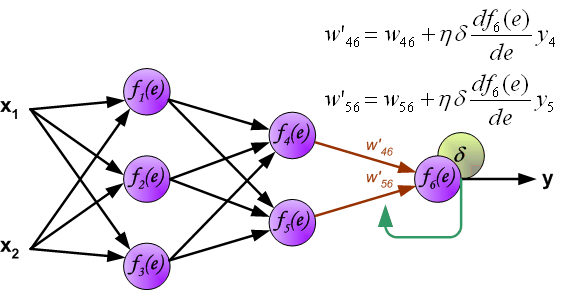
\includegraphics[scale=0.4]{img/bp.png}
    \vspace{-5pt} 
    \caption{{\tiny A 4-layer backpropagation network (Wikipedia).}}
  \end{figure}
  
  \begin{center} 
    \vspace{-5pt} 
    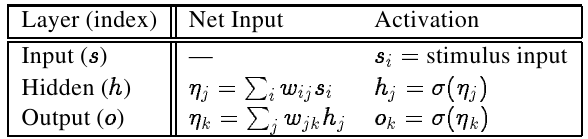
\includegraphics[scale=0.4]{img/table_bp.png}
  \end{center} 
\end{frame}

\begin{frame}{Kontext práce - GeneRec}
  \begin{itemize} 
    \item The generalized recirculation algorithm (O'Reilly 1996).
  \end{itemize} 
  
  \begin{figure}
    \centering
    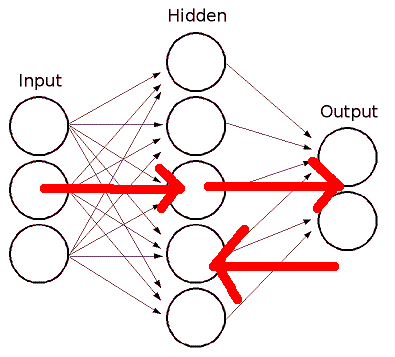
\includegraphics[scale=0.4]{img/3_layer_network_generec.png}
    %\caption{{\tiny A standard 3-layer network (Wikipedia).}} 
  \end{figure} 
  \begin{figure}  
    \centering
    \vspace{-10pt} 
    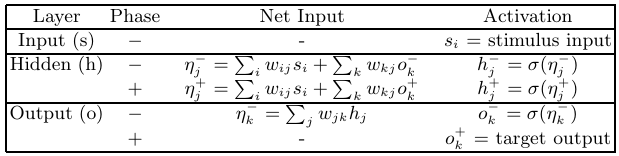
\includegraphics[scale=0.4]{img/generec_activations.png}
    \caption{{\tiny Equilibrium network variables in GeneRec model (O'Reilly, 96).}} 
  \end{figure} 
\end{frame}


%Bidirectional Activation-based Learning algorithm (BAL) shares with GeneRec
%the phase-based activations and unit types, but differs from it by the connectivity
%that allows completely bidirectional associations to be established (GeneRec
%focuses on input-to-output mapping). Unlike GeneRec, BAL uses two pairs of
%weight matrices for each activation phase. In addition, in BAL we do not use
%dynamical settling process but compute the activations in one step as described
%in Table 2.
\begin{frame}{Kontext práce - BAL}
  \begin{itemize}
    \item BAL := Bidirectional Activation-based Neural Network Learning Algorithm (Farkaš and Rebrová, 2013).
    \item Učiace pravidlo: $ \frac{1}{\epsilon}\Delta w_{ij} = a_{i}^{-}(a_{j}^{+} - a_{j}^{-}). $
  \end{itemize}
  
  \begin{figure}[h!]  
    \centering
    \vspace{-5pt} 
    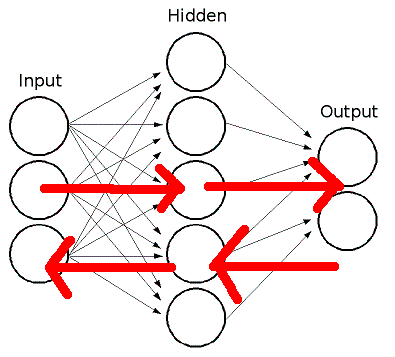
\includegraphics[scale=0.4]{img/3_layer_network_bal.png}
    %\caption{{\tiny A standard 3-layer network (Wikipedia).}} 
  \end{figure} 
  
  \begin{figure}[h!]  
    \centering
    \vspace{-5pt} 
    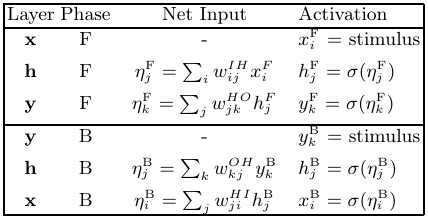
\includegraphics[scale=0.4]{img/bal_activations.png}
    \vspace{-5pt} 
    \caption{{\tiny Activation phases and states in BAL model (Farkaš and Rebrová, 2013).}} 
  \end{figure} 
\end{frame}


%%%%%%%%%%%%%%%%%%%%%%%%%%%%%%%%%%%%%%%%%%%%%%%%%%%%%%%%%%%%%%%%%%%%%%%%%
%%%%%%%%%%%%%%%%%%%%%%%%%%%%%%%%%%%%%%%%%%%%%%%%%%%%%%%%%%%%%%%%%%%%%%%%%
%V nadväznosti na úvodnú časť formulujte cieľ diplomovej práce.
%Na stránky uvádzajte malý počet riadkov.
%Vyhýbajte sa používaniu žargónu.
%Používajte starú múdrosť: 1 obrázok je viac než 1000 slov.
%%%%%%%%%%%%%%%%%%%%%%%%%%%%%%%%%%%%%%%%%%%%%%%%%%%%%%%%%%%%%%%%%%%%%%%%%
%%%%%%%%%%%%%%%%%%%%%%%%%%%%%%%%%%%%%%%%%%%%%%%%%%%%%%%%%%%%%%%%%%%%%%%%%

\begin{frame}{Cieľ diplomovej práce} 
  \begin{enumerate} 
    %\item Implement the GeneRec learning algorithm and test its properties using selected data sets.
    %\item Consider suitable modifications of the algorithm aimed at improving the network performance.
    %\item Analyse the convergence of the BAL network aimed at finding parameters on which the convergence depends. 
    \item Implementovať algoritmus GeneRec a otestovať ho na vybraných dátových vstupoch. 
    \item Zvážiť vhodné modifikácie algoritmu zamerané na výkonnosť siete. 
    \item Analyzovať model BAL a zistiť dôvody konvergencie. 
  \end{enumerate} 
  
  \begin{center}
    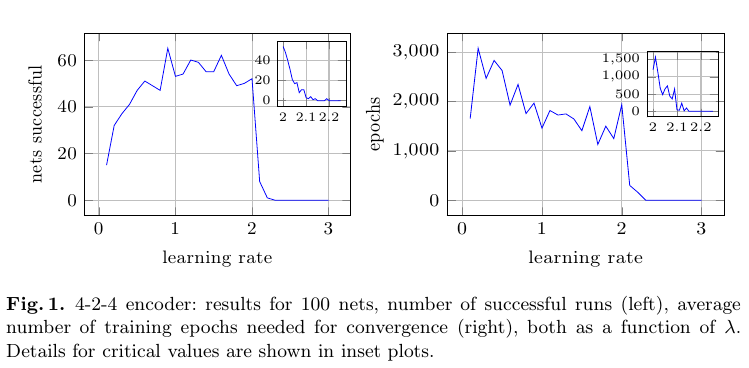
\includegraphics[scale=0.40]{img/bal_performance.png}
  \end{center}  
  
\end{frame} 

%%%%%%%%%%%%%%%%%%%%%%%%%%%%%%%%%%%%%%%%%%%%%%%%%%%%%%%%%%%%%%%%%%%%%%%%%
%%%%%%%%%%%%%%%%%%%%%%%%%%%%%%%%%%%%%%%%%%%%%%%%%%%%%%%%%%%%%%%%%%%%%%%%%
%V ďalšej časti prezentujte vlastný prínos a vlastné výsledky porovnajte s výsledkami iných. Charakterizujte použité metódy.
%Na stránky uvádzajte malý počet riadkov.
%Vyhýbajte sa používaniu žargónu.
%Používajte starú múdrosť: 1 obrázok je viac než 1000 slov.
%%%%%%%%%%%%%%%%%%%%%%%%%%%%%%%%%%%%%%%%%%%%%%%%%%%%%%%%%%%%%%%%%%%%%%%%%
%%%%%%%%%%%%%%%%%%%%%%%%%%%%%%%%%%%%%%%%%%%%%%%%%%%%%%%%%%%%%%%%%%%%%%%%%

\begin{frame}{Vlastný prínos a vlastné výsledky}
  \begin{itemize}
    \item Zrekonštruovanie výsledkov GeneRec a BAL. 
    \item Analýza mnou navrhnutých atribútov siete BAL v priebehu učenia. 
    \item Zvýšenie úspešnosti pri výbere sietí so vzdialenejšími reprezentáciami na skrytej vrstve. 
  \end{itemize} 
  
  \begin{figure}[h!]  
    \centering
    \vspace{-8pt} 
    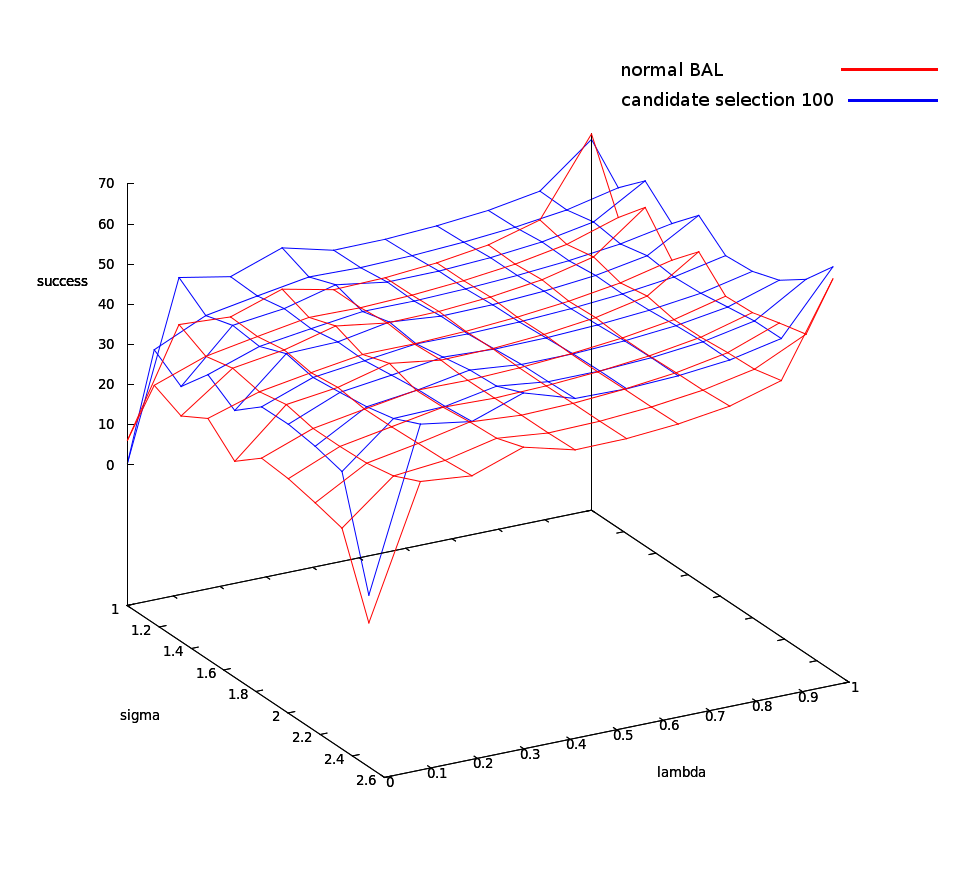
\includegraphics[scale=0.20]{img/compare_normal_and_hdist2.png}
    \caption{{\tiny $\lambda = \epsilon$ = rýchlosť učenia; $\sigma$ = disperzia normálnej distribúcie pôvodných váh}} 
  \end{figure} 
\end{frame}

%TODO legenda ku grafom 

\begin{frame}{Porovnanie s výsledkami iných}

  \begin{figure}[h!]  
    \centering
    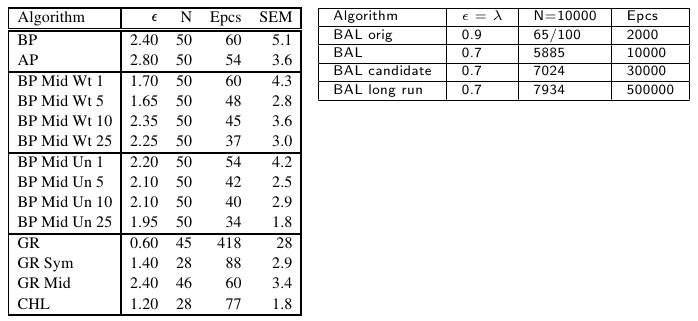
\includegraphics[scale=0.4]{img/comparison_both.png} 
%    \begin{tabular}{cc}
%        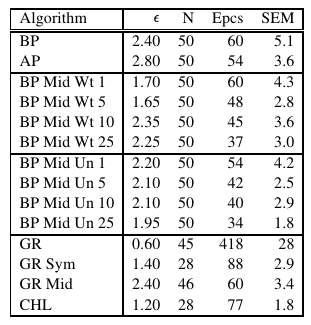
\includegraphics[scale=0.4]{img/comparison.png} 
%      & 
%        {\tiny
%        \begin{tabular}{|l|l|l|l|}
%          \hline
%          Algorithm&$\epsilon = \lambda$&N=10000&Epcs\\
%          \hline
%          BAL orig &0.9&65/100&2000\\
%         \hline
%          BAL&0.7&5885&10000\\
%          \hline
%         BAL candidate&0.7&7024&30000\\
%          \hline
%          BAL long run&0.7&7934&500000\\
%          \hline
%        \end{tabular}
%        }
%      \\
%    \end{tabular} 
    \caption{{\tiny Results for the 4-2-4 encoder problem. $\epsilon$ is the optimal learning rate, $N$ is the number of networks that successfully solved the problem (out of 50), $Epcs$ is the mean number of epochs required to reach criterion, and $SEM$ is the standard error of this mean (O'Reilly, 96).}} 
  \end{figure} 
  \begin{center}
    
  \end{center} 
\end{frame}

\begin{frame}{Použité metódy - čo nefungovalo}
  \begin{itemize}
    \item Doteraz sme vyskúšali viacero modifikácií: 
    \begin{itemize} 
      \item Momentum učenia.
      \item Dávkové učenie. 
      \item Permutácia vstupov. 
      \item Cielené generovanie počiatočných váh. 
%      \item Dropout - vynechanie niektorých skrytých neurónov. 
      \item Iné učiace pravidlá, napr. CHL symetric learning rule.
    \end{itemize} 
    \item V prípade 4-2-4 encoder-a sme dosiahli 70-75\% úspešnosť, pričom Backpropagation má 100\% úspešnosť (jednosmerne). 
  \end{itemize} 
\end{frame} 

\begin{frame}{Zobrazenie priebehu}
  \begin{figure}[h!]  
    \centering
    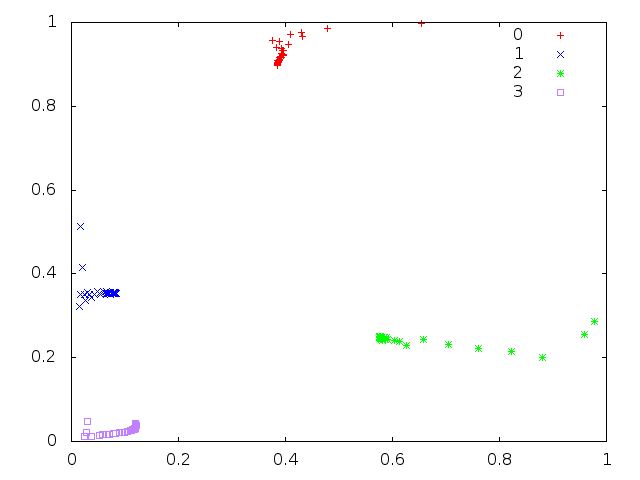
\includegraphics[scale=0.4]{img/nice.png}
    \caption{{\tiny Zobrazenie priebehu skrytých aktivácií. Táto sieť bola {\bf úspešná}.}} 
  \end{figure} 
\end{frame} 

\begin{frame}{Zobrazenie priebehu}
  \begin{figure}[h!]  
    \centering
    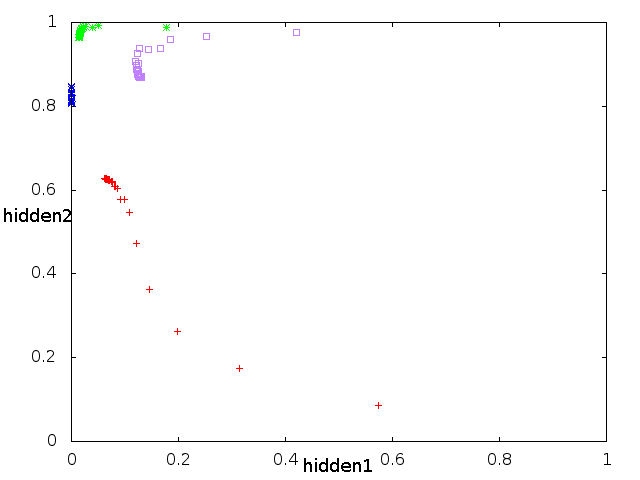
\includegraphics[scale=0.4]{img/left_top.png}
    \caption{{\tiny Zobrazenie priebehu skrytých aktivácií. Táto sieť bola {\bf úspešná}.} }
  \end{figure} 
\end{frame}

\begin{frame}{Zobrazenie priebehu}
  \begin{figure}[h!]  
    \centering
    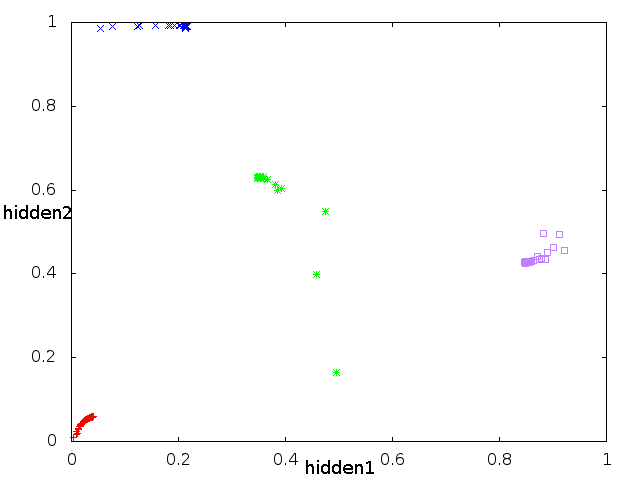
\includegraphics[scale=0.4]{img/tazisko.png}
    \caption{{\tiny Zobrazenie priebehu skrytých aktivácií. Táto sieť bola {\bf neúspešná}.} }
  \end{figure} 
\end{frame}

\begin{frame}{Zobrazenie priebehu}
  \begin{figure}[h!]  
    \centering
    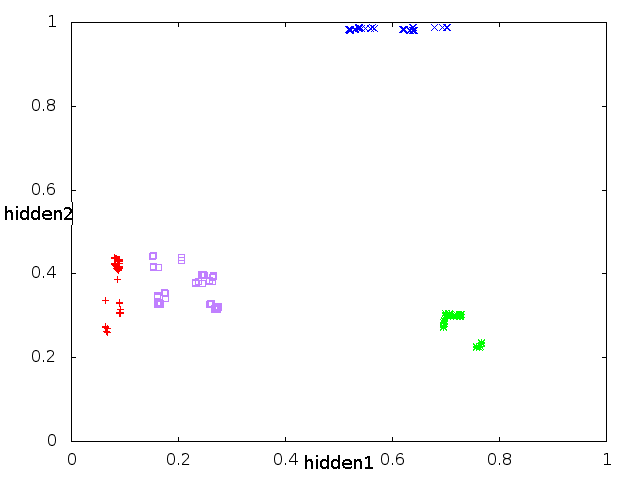
\includegraphics[scale=0.4]{img/non-convergent.png}
    \caption{{\tiny Zobrazenie priebehu skrytých aktivácií. Táto sieť bola {\bf neúspešná}.}} 
  \end{figure} 
\end{frame}


%%%%%%%%%%%%%%%%%%%%%%%%%%%%%%%%%%%%%%%%%%%%%%%%%%%%%%%%%%%%%%%%%%%%%%%%%
%%%%%%%%%%%%%%%%%%%%%%%%%%%%%%%%%%%%%%%%%%%%%%%%%%%%%%%%%%%%%%%%%%%%%%%%%
%Na záver sformulujte možnosti ďalšieho rozpracovania práce.
%Na stránky uvádzajte malý počet riadkov.
%Vyhýbajte sa používaniu žargónu.
%Používajte starú múdrosť: 1 obrázok je viac než 1000 slov.
%%%%%%%%%%%%%%%%%%%%%%%%%%%%%%%%%%%%%%%%%%%%%%%%%%%%%%%%%%%%%%%%%%%%%%%%%
%%%%%%%%%%%%%%%%%%%%%%%%%%%%%%%%%%%%%%%%%%%%%%%%%%%%%%%%%%%%%%%%%%%%%%%%%

\begin{frame}{Možnosti ďalšieho rozpracovania práce}
  \begin{itemize} 
    \item Matematická formulácia aproximácie dynamického systému BAL a skúmanie jeho konvergencie. 
    \item Učenie ako hľadanie stacionárneho bodu dynamického systému.
    \item Urýchlenie konvergencie pomocou momentumu. 
  \end{itemize} 
\end{frame} 

\begin{frame}{Priestor na otázky}
  \begin{center}
  
\includegraphics[scale=0.75]{img/question.png}
  \end{center}
%  Aktuálna verzia: \url{https://github.com/Petrzlen/diplomovka}
\end{frame}

\begin{frame}{Ďakujem za pozornosť!}
  \begin{center}
{\bf Ďakujem za pozornosť!} 
  \end{center}
  
  \vspace{3cm}
  
  \begin{center}
  \small{P.S. Ospravedlňujeme sa za kvalitu obrázkov.}
  \end{center}
\end{frame}

\end{document}

